\documentclass{beamer}
\mode<presentation> {
	\usetheme{Goettingen}
	\usecolortheme{beaver}
}
\usepackage[utf8]{inputenc} % Enforce UTF8.
\usepackage{graphicx} % Allows including images
\usepackage{booktabs} % Allows the use of \toprule, \midrule and \bottomrule in tables

%----------------------------------------------------------------------------------------
%	TITLE PAGE
%----------------------------------------------------------------------------------------

\title[Local Backprop]{Hebbian Equivelance of Backpropagation}
\author{Batuhan Başerdem}
\institute[SBU & CSHL]{
Cold Spring Harbor Labs \\ % Your institution for the title page
\medskip
\textit{bbaserde@cshl.edu} % Your email address
}
\date{\today} % Date, can be changed to a custom date

\begin{document}

\begin{frame}
\titlepage % Print the title page as the first slide
\end{frame}

\begin{frame}
\frametitle{Overview} % Table of contents slide, comment this block out to remove it
\tableofcontents % Throughout your presentation, if you choose to use \section{} and \subsection{} commands, these will automatically be printed on this slide as an overview of your presentation
\end{frame}

%----------------------------------------------------------------------------------------
%	PRESENTATION SLIDES
%----------------------------------------------------------------------------------------

%------------------------------------------------
\section{Motivation}

\begin{frame}
	\frametitle{Motivation of problem at hand}
	\begin{itemize}
		\item Preprocessing in olfactory system
		\item Dendritic connections
		\item Local algorithm vs. backpropagation
	\end{itemize}
\end{frame}

%------------------------------------------------
\section{Rundown}

\begin{frame}
	\frametitle{Network explanation}
\end{frame}

\begin{frame}
	\frametitle{ReLU}
	\begin{itemize}
		\item Rectified Linear Unit
	\end{itemize}
	\begin{figure}
		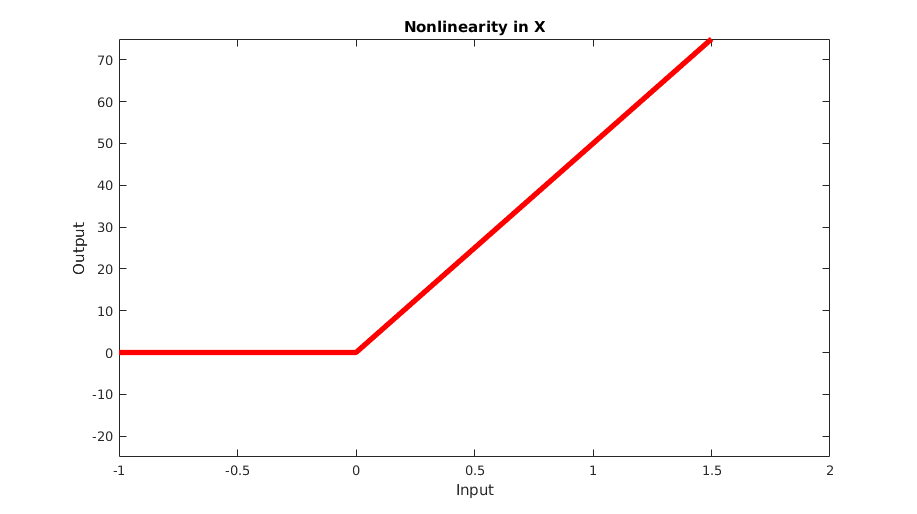
\includegraphics[width=0.9\linewidth]{plots/ReLU.png}
	\end{figure}
\end{frame}
\begin{frame}
	\frametitle{ReSU}
	\begin{itemize}
		\item Rectified Sigmoidal (or Switching) Unit
	\end{itemize}
	\begin{figure}
		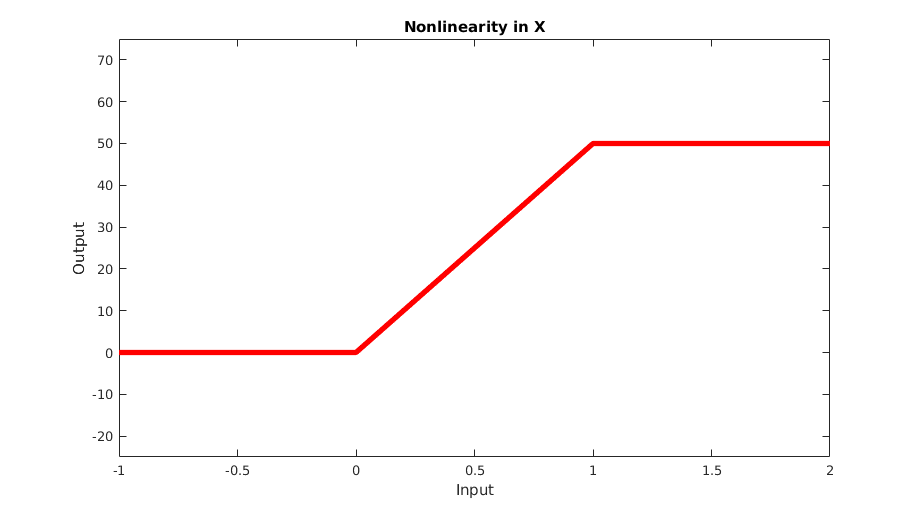
\includegraphics[width=0.9\linewidth]{plots/ReSU.png}
	\end{figure}
\end{frame}
	
%------------------------------------------------
\section{Current Results}
%\begin{figure}
%\includegraphics[width=0.9\linewidth]{test}
%\end{figure}

% 10 digits, single layer
\begin{frame}
	\frametitle{Single layer, 10 digits, results}
	\begin{itemize}
		\item Learning is happening.
	\end{itemize}
\end{frame}
\begin{frame}
	\frametitle{Single layer, 10 digits, A is fixed; Error}
	\begin{figure}
		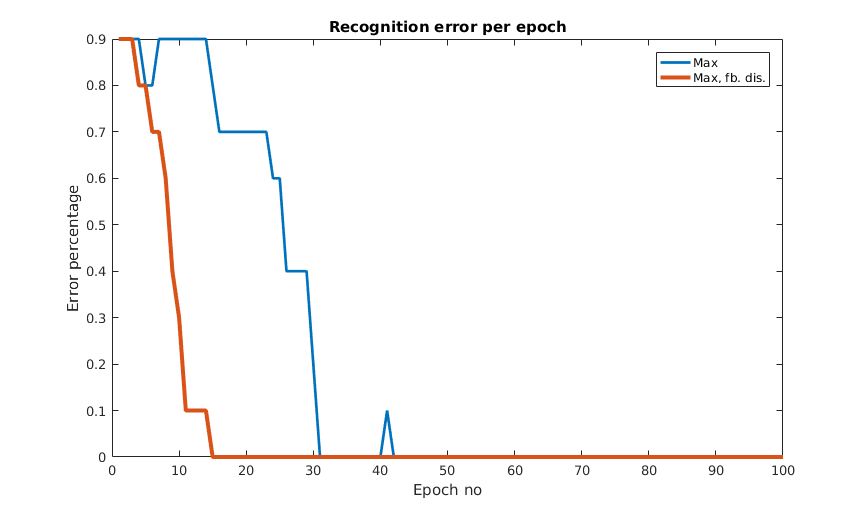
\includegraphics[width=0.9\linewidth]{plots/trn-1l-nA-error.png}
	\end{figure}
\end{frame}
\begin{frame}
	\frametitle{Single layer, 10 digits, A is fixed; Layer Average}
	\begin{figure}
		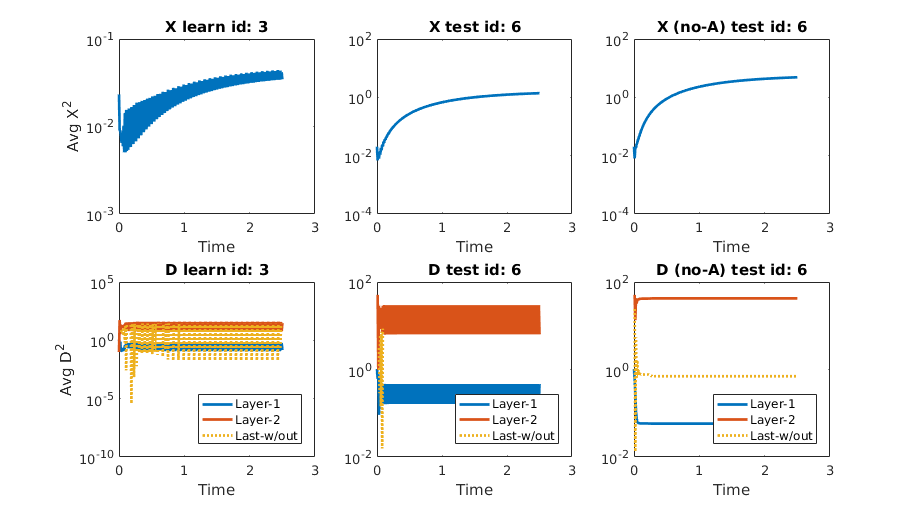
\includegraphics[width=0.9\linewidth]{plots/trn-1l-nA-av.png}
	\end{figure}
\end{frame}
\begin{frame}
	\frametitle{Single layer, 10 digits; Error}
	\begin{figure}
		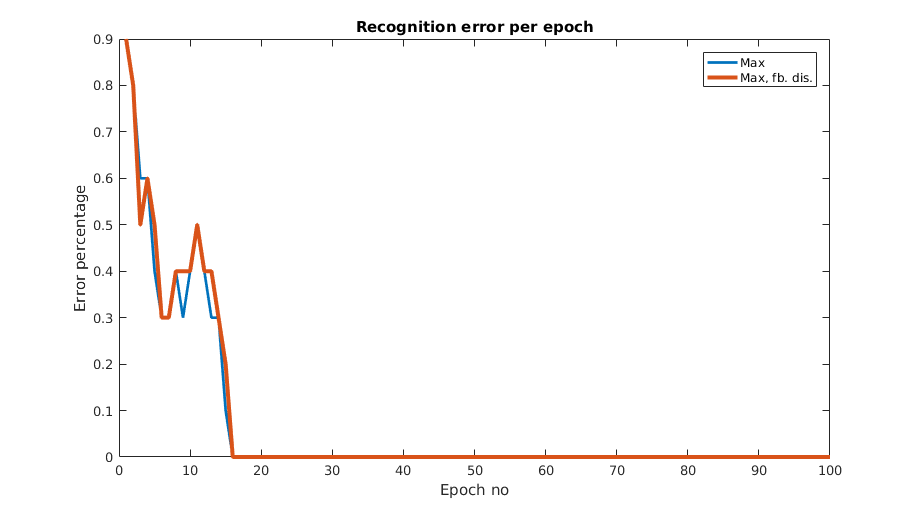
\includegraphics[width=0.9\linewidth]{plots/trn-1l-bias-error.png}
	\end{figure}
\end{frame}
\begin{frame}
	\frametitle{Single layer, 10 digits; Layer Average}
	\begin{figure}
		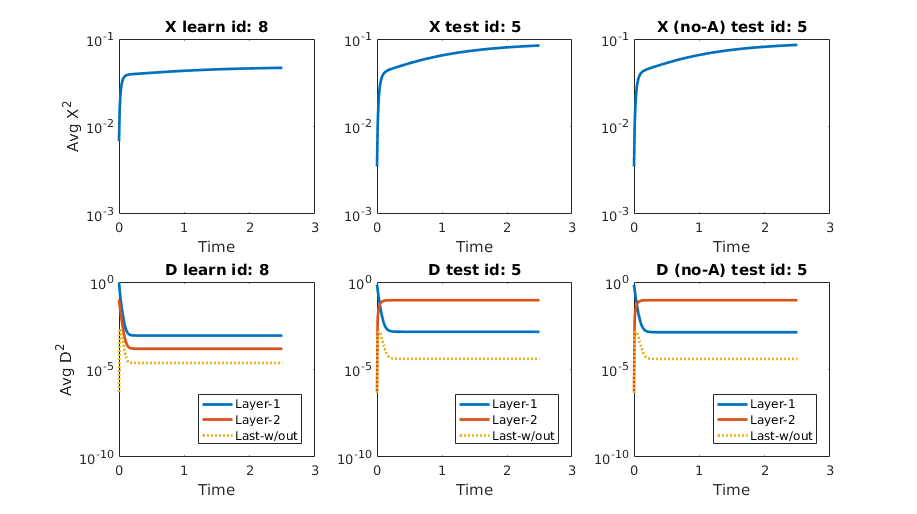
\includegraphics[width=0.9\linewidth]{plots/trn-1l-bias-average.png}
	\end{figure}
\end{frame}

% all digits, single layer
\begin{frame}
	\frametitle{Single layer, entire MNIST dataset, results}
	\begin{itemize}
		\item Better results when last layer feedback to X is blocked
		\item Better results when A layer is fixed to identity
		\item Initial hurdle with error rate going up is decreased
		\item Biasing rules work, but no improvement over performance
		\item ReLU and ReSU similar performance
	\end{itemize}
\end{frame}
\begin{frame}
	\frametitle{Single layer, example; parameters}
	\begin{itemize}
		\item A is fixed at identity.
		\item Bias is learned
		\item Steepness is 10
		\item Learning rate is $5 \times 10^{-8}$
		\item Learning rate not adaptive
		\item Weight decay is not used
		\item Simulation time = 2
		\item simulation time steps = 0.007
		\item Nonlinearity = ReLU
	\end{itemize}
\end{frame}
\begin{frame}
	\frametitle{Single layer, example; errors}
	\begin{figure}
		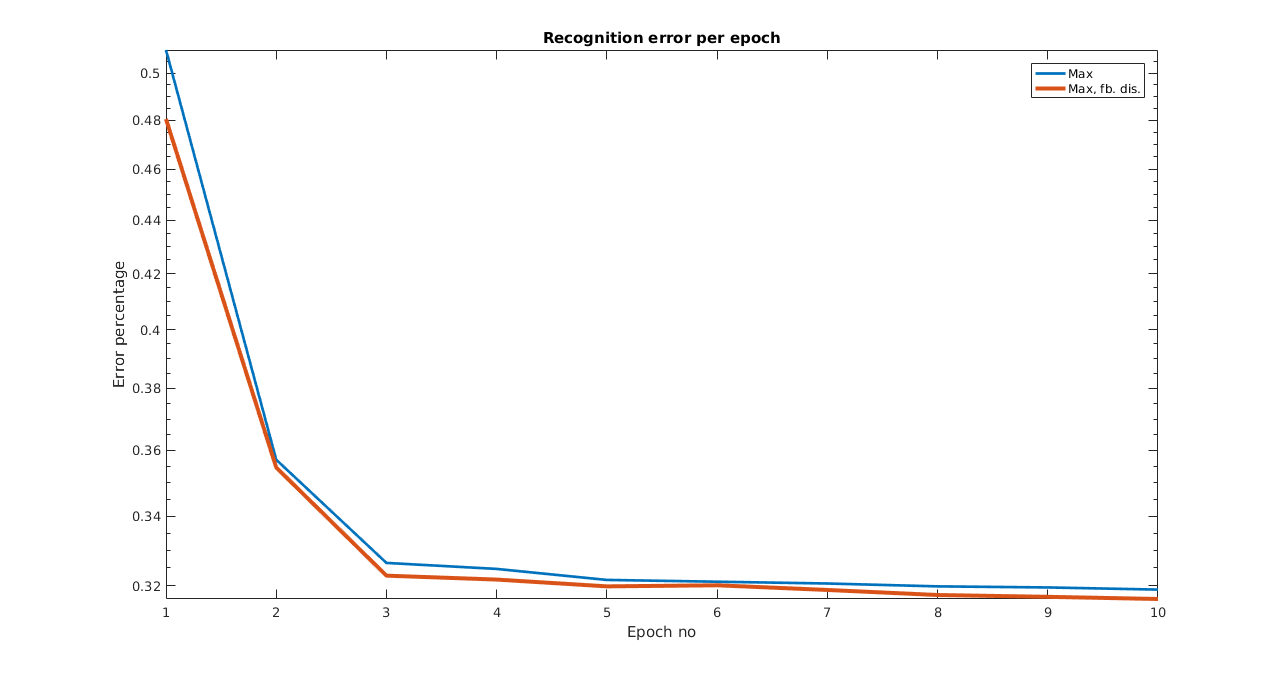
\includegraphics[width=0.9\linewidth]{plots/full_1l_nA_errors.png}
	\end{figure}
\end{frame}
\begin{frame}
	\frametitle{Single layer, example; averages}
	\begin{figure}
		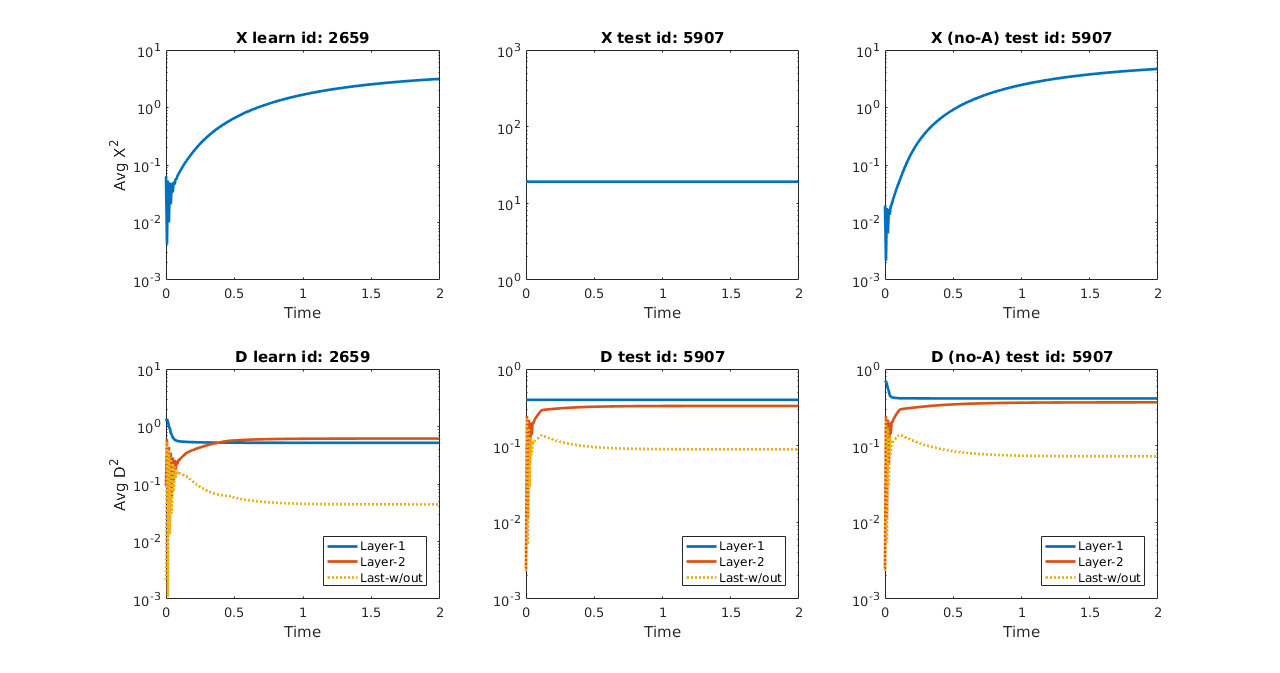
\includegraphics[width=0.9\linewidth]{plots/full_1l_nA_average.png}
	\end{figure}
\end{frame}

% 10 digits dual layer
\begin{frame}
	\frametitle{Dual layer, entire MNIST dataset}
	\begin{itemize}
		\item Better results when last layer feedback to X is blocked
		\item Better results when A layer is fixed to identity
	\end{itemize}
\end{frame}
%------------------------------------------------
\end{document} 